\documentclass[10pt,a4paper]{article}
\usepackage[a4paper]{geometry}
\usepackage[english]{babel}
\usepackage{amsmath}
\usepackage{amsfonts}
\usepackage{amssymb}
\usepackage{makeidx}
\usepackage{graphicx}
\usepackage{caption}
\usepackage{subcaption}
\usepackage{color}
\usepackage{import}

\usepackage{float}

\usepackage{pdfpages}

\usepackage{epstopdf}

\usepackage{hyperref}

\title{TP Morphologie math\'{e}matiques : les op\'{e}rateurs \'{e}l\'{e}mentaires et leurs applications}
\author{} %, \href{mailto:matthew.ozon@cpe.fr}{matthew.ozon@cpe.fr}
\date{\today}

%begining of the document
\begin{document}
\maketitle

\section{introduction} 
\paragraph{Rappel}
Avant tout, nous vous rappelons, m\^{e}me si ce n'est pas n\'{e}cessaire, que la documentation et des exemples consernant les fonctions que vous allez utiliser est disponnible soit dans le logiciel via la commande \textit{help} soit en cherchant sur le web via votre moteur de recherche pr\'{e}f\'{e}rer. 

\subsection{Objectif}
Ce premier TP du module de TSI vous permet de vous familiariser avec :
\begin{itemize}
	\item la manipulation des donn\'{e}es images via les fonctions de chargement comme \textit{imread}, l'affichage \textit{imshow} ou histogramme comme \textit{hist} et bien d'autres.
	\item les op\'{e}rateurs \'{e}l\'{e}mentaire de morphologie math\'{e}matiques
	\item des applications un peu plus avanc\'{e}es se basant sur les op\'{e}rateurs d’\'{e}rosion, dilatation, ouverture et fermeture.
\end{itemize}

\subsection{\`{A} rendre}
De votre part, nous attendons deux \'{e}l\'{e}ments : 
\begin{itemize}
	\item Un compte rendu expliquant votre d\'{e}marche, vos codes : il faut que vous montriez que vous avez compris de quoi il s'agit de fa\c{}on concise (8 pages maximum sans les figures)
	\item Des script : un pour chaque question avec des figures si n\'{e}cessaire (toujours comment\'{e}es)
\end{itemize}

\subsection{Les moyens}
Vous trouverez toutes les ressources (r\'{e}sume de cours, \'{e}nonc\'{e} de TP et des morceaux de script \`{a} compl\'{e}ter) \`{a} l'adresse suivante : \url{https://github.com/matthewozon/TPmorphoMath4ETI}

\noindent\textbf{Consigne \`{a} observer} Le TP doit se d\'{e}rouler sous OCTAVE que vous pouvez lancer soit en mode terminal via la commande \textit{octave} soit en d\'{e}marrant l'interface graphique \textit{QtOctave}.

%Respecter la hierachie des fichiers. 

\paragraph{conseil pour les figures} Utiliser la commande  \textit{print(`-depsc',`nom\_du\_fichier')}  qui ``imprime'' ce que vous voyez dans la figure sans en diminuer la qualit\'{e} (contrairement au capture d’\'{e}cran). Pour plus d'information sur cette commande, nous vous invitons a taper dans votre prompt octave \textit{help print}.

\paragraph{autre conseil} Vous allez utiliser des images binaires, pensez a vous servir des op\'{e}rations logique comme : \textit{and}, \textit{or}, \textit{not}, \textit{xor}, etc.




\section{Prise en main}
Dans cette section vous allez voir comment faire pour acc\'{e}der aux donn\'{e}es d'une image et la transformer. Commencez par cr\'{e}er un fichier ``TP\_moprho\_init.m'' qui commencera par les trois lignes suivantes : 
\begin{itemize}
	\item[] clc
	\item[] clear all
	\item[] close all
\end{itemize}
pour \'{e}viter d'avoir des conflit de d\'{e}finition et des affichages multiple en navigant entre les fichiers.

\subsection{Affichage d'une image}
Testez le script suivant et d\'{e}crivez ce qu'il fait. Apportez des modifications si n\'{e}cessaire.

\begin{verbatim}
clear all;
close all;
clc;

%chargement de l'image dans un tableau
imRGB = imread('accessoire_poker_heart.jpg');

%affichage de l'image
figure(1)
imshow(imRGB)
title('mon titre')

%autre methode d'affichage
figure(2)
imagesc(imRGB)
title('mon autre titre')
%colormap jet %ligne a decommenter pour tester
%colorbar

%transformation de l'image en niveau de gris methode 1
class(imRGB(1)) %affiche le type de variable
imGray1 = imRGB(:,:,1) + imRGB(:,:,2) + imRGB(:,:,3); %somme des trois composantes... mais est-ce correcte?

%transformation de l'image en niveau de gris methode 2
imGray2 = rgb2gray(imRGB);

figure(3)
subplot(121)
imshow(imGray1)
title('methode de transformation : somme des composantes')
subplot(122)
imshow(imGray2)
title('methode de transformation : commande rgb2gray')

\end{verbatim}




\subsection{Binarisation}

Maintenant que vous savez charger une image en m\'{e}moire et que vous pouvez la transformer en niveaux de gris, vous allez chercher \`{a} binariser une image et \`{a} extraire des contours. Vous utiliserez le script suivant en apportant les modifications n\'{e}cessaires et vous expliquerez ce que fait le script.

\begin{verbatim}
clear all;
close all;
clc;

%chargement de l'image dans un tableau
imRGB = imread('accessoire_poker_heart.jpg'); %faut il changer de type...

%transformation de l'image en niveau de gris
imGray = ...;

%detection des contours par seuillage de la norme du gradient (estimation par filtre de sobel)
    %definition des filtre pour l'estimation du gradient
Fl = (1/4)*[-1 -2 -1;
         0   0   0;
         1   2   1];
Fc = Fl';
    %estimation des composantes du gradient
imGradl = conv2(imGray, Fl,'same');
imGradc = conv2(imGray, Fc,'same');

    %calcul de la norme du gradient
imGradNorm = ...;

    %seuillage de la norme du gradient pour extraction des contours
        %pour savoir a quelle valeur seuiller, on affiche l'histogramme de l'image a l'aide de la commande imhist
imhist...
        %pour fixer le seuil, on choisit de demander a l'utilisateur le taper dans le prompt
seuil = input("nom text\n")
        %seuillage de la norme du gradient (pas de boucle autorisee)
imGradBin = ...;

%affichage des resultats
figure(1)
...


\end{verbatim}



\clearpage
\section{Observation des op\'{e}rateurs de base}
\subsection{Somme et soustraction de Minkowski}
En vous aidant des notes de cours (mopho\_resume\_cours.pdf) et des fichier minkowskiSum.m et minkowskiSub.m, vous impl\'{e}menterez les op\'{e}rations d'addition et de soustraction Minkowskiennes. Attention, votre code ne doit pas contenir plus de deux boucles \textbf{for}. Vous testerez vos impl\'{e}mentations sur des \'{e}l\'{e}ments simple comme un cercle avec un carre. 

\noindent\textbf{Attention} : ces deux codes sont tr\`{e}s importants car toutes les autres parties reposent dessus, il faut donc que vous pr\^{e}tiez une attention toute particuli\`{e}re \`{a} la validation de cette \'{e}tape. 

\noindent\textbf{Conseil} : pour la validation, vous pouvez cr\'{e}er des objet simple comme le disque centre sur l'origine et de rayon 5 que r\'{e}alise le script suivant.
\begin{verbatim}
[dC,dL] = meshgrid(-49:50,-49:50);
X = sqrt(dC.^2 + dL.^2)<5;
\end{verbatim}

\noindent\textbf{\`{A} rendre} : explication du script et de sa validation.


\subsection{\'{E}rosion, dilatation, ouverture et fermeture}
\textbf{Impl\'{e}mentation} Impl\'{e}mentez les op\'{e}rateurs d'\'{e}rosion et de dilatation a l'aide des somme et soustraction de Minkowski. Impl\'{e}mentez ensuite l'ouverture et la fermeture en utilisant les op\'{e}rateur que vous venez de coder.

\noindent\textbf{Validation} Dans une premier temps, tester vos algorithmes sur les images qui vous sont fournis (certaine sont binaire comme ``veau2\_moins\_petit.bmp'' et peuvent \^{e}tre utilis\'{e}es sans pr\'{e}-traitement). Vous pouvez aussi comparer vos r\'{e}sultats \`{a} ceux des fonctions \textit{imerode}, \textit{imdilate}, \textit{imopen} et \textit{imclose}.

\noindent\textbf{\`{A} rendre} : Test de plusieurs \'{e}l\'{e}ments structurants sur une image de votre choix dans le jeu d'images fournis. Mise en \'{e}vidence des propri\'{e}t\'{e}s de composition et de dualit\'{e} pour \'{e}rosion/dilatation et propri\'{e}t\'{e}s d'idempotence et de dualit\'{e} pour  ouverture/fermeture. Faire le lien entre la dilatation et le seuillage de la carte de distance. Proposez solution similaire pour l'\'{e}rosion.

\subsection{Hit or Miss}
\textbf{Impl\'{e}mentation} En utilisant les op\'{e}rateurs pr\'{e}c\'{e}demment cod\'{e}s, impl\'{e}mentez la transform\'{e}e Tout-ou-Rien.

\noindent\textbf{Validation} vous testerez sur l'image ``bin.png'' en ajoutant du bruit (des points al\'{e}atoirement distribues pour lesquels l'\'{e}tat du pixel est compl\'{e}ment\'{e}) puis en la d\'{e}bruitant. Indication : utilisez \begin{verbatim} N = randn(300,400)>2.0;\end{verbatim} pour g\'{e}n\'{e}rer le bruit et la commande \textit{xor} pour ajouter le bruit a l'image. Vous pourrez comparer votre r\'{e}sultat \`{a} celui de \textbf{bwhitmiss}.

\noindent\textbf{\`{A} rendre} : la preuve en image que votre impl\'{e}mentation fonctionne avec une explication de la m\'{e}thode que vous utilisez pour d\'{e}bruiter l'image.

\clearpage
\section{Applications}
L'id\'{e}e de cette partie est de mettre en oeuvre votre travail a des situations un peu plus complexe.
\subsection{D\'{e}tection de p\'{e}riode}
\textbf{Consigne} : utilisez l'image ``rayure.jpg'' et un \'{e}l\'{e}ment structurant forme d'une paire de points pour d\'{e}terminer la p\'{e}riode du motif.

\noindent\textbf{\`{A} rendre} : estimation de la p\'{e}riode, explication de votre m\'{e}thode et la preuve en image.

\subsection{Granulom\'{e}trie}
\textbf{Consigne} : utilisez l'image (tout ou partie) ``NGC6960\_24Juillet2006\_LD.jpg'' et tracez la courbe granulometrique pour deux \'{e}l\'{e}ments structurants de votre choix.

\noindent\textbf{\`{A} rendre} : explication de la m\'{e}thode et illustration.


\subsection{Comptage de trou}
\textbf{Consigne} : A partir du script suivant qui g\'{e}n\`{e}re un disque perce de plusieurs trou, compter le nombre de trou. Indication : servez vous du nombre de connexit\'{e}s.
\begin{verbatim}
%creation d'un grand disque centre sur le centre de l'image
[dC,dL] = meshgrid(-49:50,-49:50);
imBin = sqrt(dC.^2 + dL.^2)<43;

%creation de composantes a enlever du disque
composanteConnex = (sqrt((dC+5).^2 + dL.^2)<5) | (sqrt(dC.^2 + (dL+10).^2)<5) | (sqrt((dC-15).^2 + dL.^2)<5) | (sqrt((dC+25).^2 + dL.^2)<5) | (sqrt(dC.^2 + (dL-20).^2)<5) | (sqrt(dC.^2 + (dL+30).^2)<5);

%ajout des composantes
imBin = and(imBin,not(composanteConnex));
\end{verbatim}
Essayer de compter le nombre de trou sur le disque de frein ``disque\_frein\_bin.tif''.

\noindent\textbf{\`{A} rendre} : expliquer votre m\'{e}thode.

\subsection{Gradient... comparaison avec Hit-or-Miss}
\textbf{Consigne} : Impl\'{e}mentez le gradient morphologique et le tester sur un image de votre choix. Proposez une alternative avec la transform\'{e}e Tout-ou-Rien. Comparer les deux r\'{e}sultats.

\noindent\textbf{\`{A} rendre} : expliquer votre m\'{e}thode et commenter vos r\'{e}sultats.

\subsection{Squelette}
\textbf{Consigne} : squelettisez le petit veau! (A l'aide de votre propre m\'{e}thode)

\noindent\textbf{\`{A} rendre} : Le squelette et son  tueur!





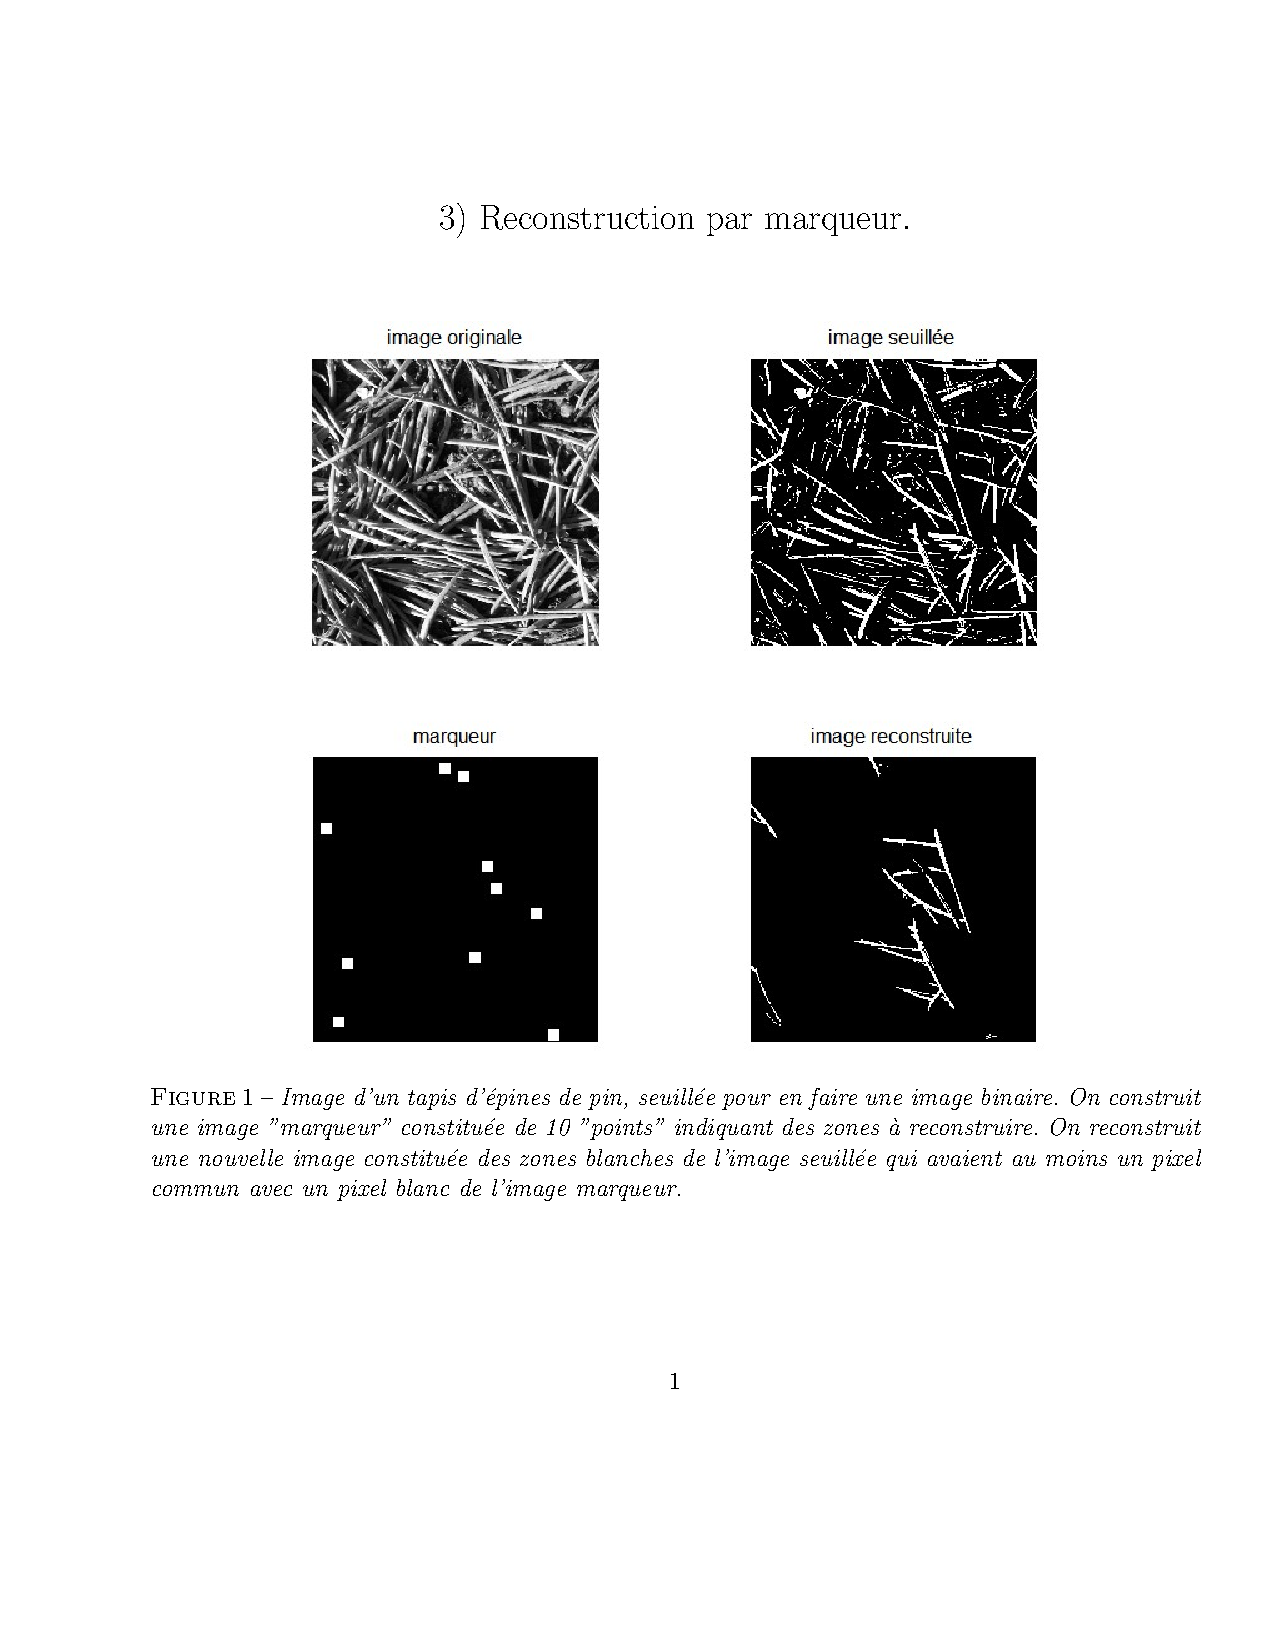
\includepdf[pages={-}]{ContributionTP1.pdf}


\end{document}





